\documentclass[a4paper, 10pt]{article}
\usepackage[margin=0.5in]{geometry}

\usepackage{blindtext}
\usepackage{multicol}
\usepackage{booktabs}
\usepackage{amsmath}
\usepackage{mathtools}
\usepackage{float}
\usepackage{graphicx}
\usepackage{enumitem}
\usepackage{hyperref}
\usepackage{comment}

\graphicspath{ {../outputs/}{../data/} }


\setlength{\columnsep}{1cm}
\title{ENPM 673: Perception for Autonomous Robots - Project 2}
\author{Aswath Muthuselvam \\ aswath@umd.edu}
\date{18th April 2022}

\begin{document}
	\maketitle
	\newlist{contract}{enumerate}{10}
	\setlist[contract]{label*=\arabic*.}
	\setlistdepth{10} 
	
	\begin{figure}[b]
		\centering
		%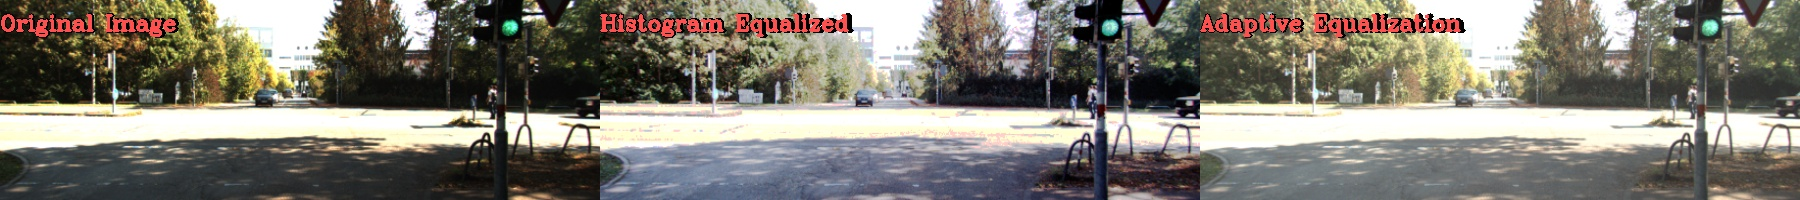
\includegraphics[width=\textwidth]{/histogram_and_adaptive.jpg}
		\caption{Original Image(left), Histogram Equalization(middle) and Adaptive Equalization(right)}
		\label{fig:HistEQ}
	\end{figure}
	
	\begin{multicols}{2}
		
		\section{Calibration}
		
		
		\begin{equation} \label{eq:gamma}
		I_{out}=I_{in}^{\gamma}
		\end{equation}
		
		\section{Rectification}
		
		
		\begin{figure}[H]
			\centering
			%\includegraphics[width=\columnwidth]{/straight_lane_segments.png}
			\caption{Lane detection: red line markings for road boundary, right lane for green markings. Purple circle shows the vanishing point found by the intersecting lanes.}
			\label{fig:straight_segments}
		\end{figure}
		
		A video preview of the lane segment detection method is available in this \href{https://youtu.be/6CWymeqQOWk}{YouTube link}, and the lane detection method is available in this \href{https://youtu.be/fkf3r3iCl74}{YouTube link}.
		
		\section{Correspondence}	
		
		
		A video preview of the curve lane detection method is available in this \href{https://youtu.be/5v3jpyDuoz4}{YouTube link}.
		
		
		
		\section{Compute Depth Image}
		
		
		\section{Conclusion}	
		
		
	\end{multicols}
	
	
	
\end{document}
